% Options for packages loaded elsewhere
\PassOptionsToPackage{unicode}{hyperref}
\PassOptionsToPackage{hyphens}{url}
\PassOptionsToPackage{dvipsnames,svgnames,x11names}{xcolor}
%
\documentclass[
  ignorenonframetext,
]{beamer}
\usepackage{pgfpages}
\setbeamertemplate{caption}[numbered]
\setbeamertemplate{caption label separator}{: }
\setbeamercolor{caption name}{fg=normal text.fg}
\beamertemplatenavigationsymbolsempty
% Prevent slide breaks in the middle of a paragraph
\widowpenalties 1 10000
\raggedbottom

\usepackage{amsmath,amssymb}
\usepackage{iftex}
\ifPDFTeX
  \usepackage[T1]{fontenc}
  \usepackage[utf8]{inputenc}
  \usepackage{textcomp} % provide euro and other symbols
\else % if luatex or xetex
  \usepackage{unicode-math}
  \defaultfontfeatures{Scale=MatchLowercase}
  \defaultfontfeatures[\rmfamily]{Ligatures=TeX,Scale=1}
\fi
\usepackage{lmodern}
\usetheme[]{AnnArbor}
\usecolortheme{dolphin}
\usefonttheme{structurebold}
\ifPDFTeX\else  
    % xetex/luatex font selection
\fi
% Use upquote if available, for straight quotes in verbatim environments
\IfFileExists{upquote.sty}{\usepackage{upquote}}{}
\IfFileExists{microtype.sty}{% use microtype if available
  \usepackage[]{microtype}
  \UseMicrotypeSet[protrusion]{basicmath} % disable protrusion for tt fonts
}{}
\makeatletter
\@ifundefined{KOMAClassName}{% if non-KOMA class
  \IfFileExists{parskip.sty}{%
    \usepackage{parskip}
  }{% else
    \setlength{\parindent}{0pt}
    \setlength{\parskip}{6pt plus 2pt minus 1pt}}
}{% if KOMA class
  \KOMAoptions{parskip=half}}
\makeatother
\usepackage{xcolor}
\newif\ifbibliography
\setlength{\emergencystretch}{3em} % prevent overfull lines
\setcounter{secnumdepth}{-\maxdimen} % remove section numbering


\providecommand{\tightlist}{%
  \setlength{\itemsep}{0pt}\setlength{\parskip}{0pt}}\usepackage{longtable,booktabs,array}
\usepackage{calc} % for calculating minipage widths
\usepackage{caption}
% Make caption package work with longtable
\makeatletter
\def\fnum@table{\tablename~\thetable}
\makeatother
\usepackage{graphicx}
\makeatletter
\def\maxwidth{\ifdim\Gin@nat@width>\linewidth\linewidth\else\Gin@nat@width\fi}
\def\maxheight{\ifdim\Gin@nat@height>\textheight\textheight\else\Gin@nat@height\fi}
\makeatother
% Scale images if necessary, so that they will not overflow the page
% margins by default, and it is still possible to overwrite the defaults
% using explicit options in \includegraphics[width, height, ...]{}
\setkeys{Gin}{width=\maxwidth,height=\maxheight,keepaspectratio}
% Set default figure placement to htbp
\makeatletter
\def\fps@figure{htbp}
\makeatother
% definitions for citeproc citations
\NewDocumentCommand\citeproctext{}{}
\NewDocumentCommand\citeproc{mm}{%
  \begingroup\def\citeproctext{#2}\cite{#1}\endgroup}
\makeatletter
 % allow citations to break across lines
 \let\@cite@ofmt\@firstofone
 % avoid brackets around text for \cite:
 \def\@biblabel#1{}
 \def\@cite#1#2{{#1\if@tempswa , #2\fi}}
\makeatother
\newlength{\cslhangindent}
\setlength{\cslhangindent}{1.5em}
\newlength{\csllabelwidth}
\setlength{\csllabelwidth}{3em}
\newenvironment{CSLReferences}[2] % #1 hanging-indent, #2 entry-spacing
 {\begin{list}{}{%
  \setlength{\itemindent}{0pt}
  \setlength{\leftmargin}{0pt}
  \setlength{\parsep}{0pt}
  % turn on hanging indent if param 1 is 1
  \ifodd #1
   \setlength{\leftmargin}{\cslhangindent}
   \setlength{\itemindent}{-1\cslhangindent}
  \fi
  % set entry spacing
  \setlength{\itemsep}{#2\baselineskip}}}
 {\end{list}}
\usepackage{calc}
\newcommand{\CSLBlock}[1]{\hfill\break\parbox[t]{\linewidth}{\strut\ignorespaces#1\strut}}
\newcommand{\CSLLeftMargin}[1]{\parbox[t]{\csllabelwidth}{\strut#1\strut}}
\newcommand{\CSLRightInline}[1]{\parbox[t]{\linewidth - \csllabelwidth}{\strut#1\strut}}
\newcommand{\CSLIndent}[1]{\hspace{\cslhangindent}#1}

\usepackage{booktabs}
\usepackage{longtable}
\usepackage{array}
\usepackage{multirow}
\usepackage{wrapfig}
\usepackage{float}
\usepackage{colortbl}
\usepackage{pdflscape}
\usepackage{tabu}
\usepackage{threeparttable}
\usepackage{threeparttablex}
\usepackage[normalem]{ulem}
\usepackage{makecell}
\usepackage{xcolor}

% logo
\titlegraphic{
\includegraphics[width=4cm]{000_logos/logo-blue-vertical}}
\logo{\ifnum\thepage>1
\includegraphics[width=0.5cm]{000_logos/logo-blue-vertical}\fi}

% UMNG: Manual de image institucional

% Colors

% Umng
\definecolor{yellow}{HTML}{fdc600}
\definecolor{red-dark}{HTML}{841e35}

% Estudios a Distancia
\definecolor{blue1}{HTML}{12245b}
\definecolor{blue2}{HTML}{767ca6}
\definecolor{blue3}{HTML}{cad2ec}

% Modify items
\setbeamercolor{palette primary}{bg=blue3}
\setbeamercolor{palette tertiary}{bg=blue1}
\setbeamercolor{frametitle}{bg=yellow}

% Hyperlinks
\hypersetup{
  linkcolor=red-dark,
  citecolor=red-dark
}

\makeatletter
\@ifpackageloaded{caption}{}{\usepackage{caption}}
\AtBeginDocument{%
\ifdefined\contentsname
  \renewcommand*\contentsname{Table of contents}
\else
  \newcommand\contentsname{Table of contents}
\fi
\ifdefined\listfigurename
  \renewcommand*\listfigurename{List of Figures}
\else
  \newcommand\listfigurename{List of Figures}
\fi
\ifdefined\listtablename
  \renewcommand*\listtablename{List of Tables}
\else
  \newcommand\listtablename{List of Tables}
\fi
\ifdefined\figurename
  \renewcommand*\figurename{Figure}
\else
  \newcommand\figurename{Figure}
\fi
\ifdefined\tablename
  \renewcommand*\tablename{Table}
\else
  \newcommand\tablename{Table}
\fi
}
\@ifpackageloaded{float}{}{\usepackage{float}}
\floatstyle{ruled}
\@ifundefined{c@chapter}{\newfloat{codelisting}{h}{lop}}{\newfloat{codelisting}{h}{lop}[chapter]}
\floatname{codelisting}{Listing}
\newcommand*\listoflistings{\listof{codelisting}{List of Listings}}
\makeatother
\makeatletter
\makeatother
\makeatletter
\@ifpackageloaded{caption}{}{\usepackage{caption}}
\@ifpackageloaded{subcaption}{}{\usepackage{subcaption}}
\makeatother

\ifLuaTeX
\usepackage[bidi=basic]{babel}
\else
\usepackage[bidi=default]{babel}
\fi
\babelprovide[main,import]{english}
% get rid of language-specific shorthands (see #6817):
\let\LanguageShortHands\languageshorthands
\def\languageshorthands#1{}
\ifLuaTeX
  \usepackage{selnolig}  % disable illegal ligatures
\fi
\usepackage{bookmark}

\IfFileExists{xurl.sty}{\usepackage{xurl}}{} % add URL line breaks if available
\urlstyle{same} % disable monospaced font for URLs
\hypersetup{
  pdftitle={Production and Income I},
  pdfauthor={Luis Francisco Gómez López},
  pdflang={en},
  colorlinks=true,
  linkcolor={Maroon},
  filecolor={Maroon},
  citecolor={Blue},
  urlcolor={Blue},
  pdfcreator={LaTeX via pandoc}}


\title{Production and Income I}
\author{Luis Francisco Gómez López}
\date{2024-07-13}
\institute{FAEDIS}

\begin{document}
\frame{\titlepage}

\renewcommand*\contentsname{Table of contents}
\begin{frame}[allowframebreaks]
  \frametitle{Table of contents}
  \tableofcontents[hideallsubsections]
\end{frame}

\section{Please Read Me}\label{please-read-me}

\begin{frame}{}
\phantomsection\label{section}
\begin{itemize}
\item
  Check the message \textbf{Welcome greeting} published in the News
  Bulletin Board.
\item
  Dear student please edit your profile uploading a photo where your
  face is clearly visible.
\item
  The purpose of the virtual meetings is to answer questions and not to
  make a summary of the study material.
\item
  This presentation is based on
  (\citeproc{ref-cardenas_introduccion_2020}{Cardenas 2020, chap. 2})
\end{itemize}
\end{frame}

\section{Purpose}\label{purpose}

\begin{frame}{}
\phantomsection\label{section-1}
Understand how production is measured using the concept of Gross
Domestic Product (GDP)
\end{frame}

\section{Gross Domestic Product (GDP)}\label{gross-domestic-product-gdp}

\begin{frame}{}
\phantomsection\label{section-2}
\begin{itemize}
\item
  What is? (\citeproc{ref-lequiller_understanding_2014}{Lequiller and
  Blades 2014, 19})

  \begin{itemize}
  \tightlist
  \item
    \textbf{Product}: means that we are trying to measure production
    without double counting
  \end{itemize}
\end{itemize}

\begin{center}
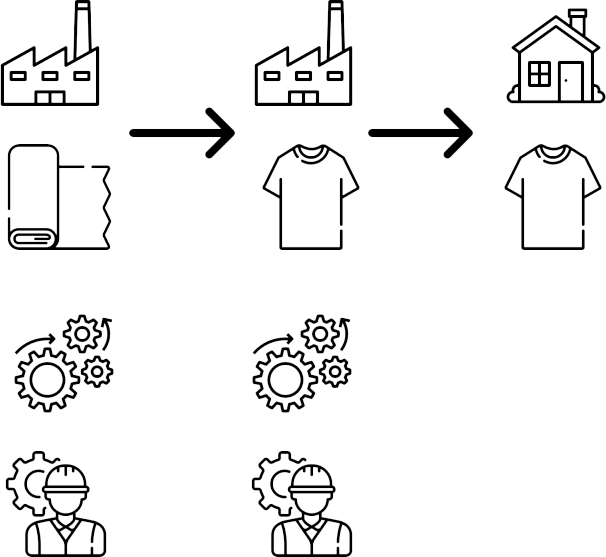
\includegraphics[width=0.4\textwidth,height=\textheight]{_000_images/001_image1.png}
\end{center}
\end{frame}

\begin{frame}{}
\phantomsection\label{section-3}
\begin{itemize}
\item
  What is? (\citeproc{ref-lequiller_understanding_2014}{Lequiller and
  Blades 2014, 19})

  \begin{itemize}
  \tightlist
  \item
    \textbf{Domestic}: means that the production to be taken into
    account is the one that is carried within a certain territory
    clearly delimited
  \end{itemize}
\end{itemize}

\begin{center}
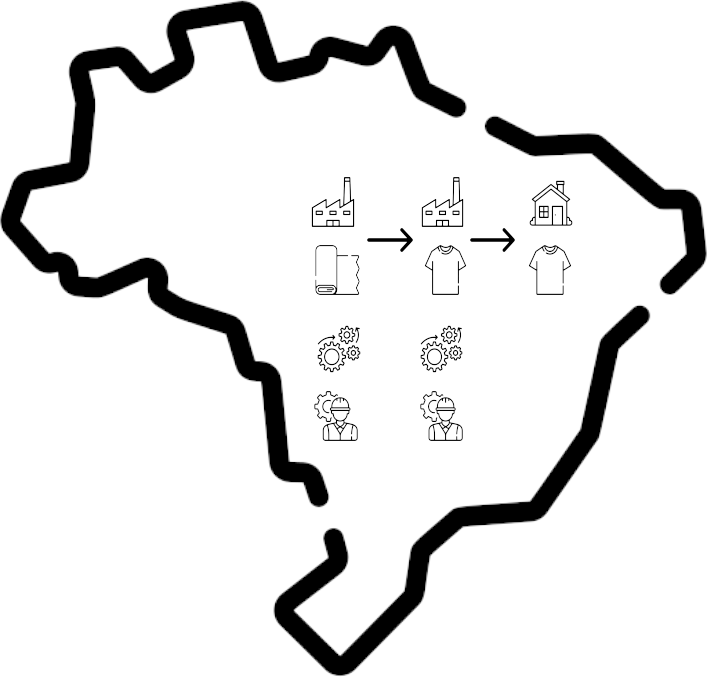
\includegraphics[width=0.45\textwidth,height=\textheight]{_000_images/001_image2.png}
\end{center}
\end{frame}

\begin{frame}{}
\phantomsection\label{section-4}
\begin{itemize}
\item
  What is? (\citeproc{ref-lequiller_understanding_2014}{Lequiller and
  Blades 2014, 19})

  \begin{itemize}
  \tightlist
  \item
    \textbf{Gross}: means that depreciation is not deducted (in economy
    it is called consumption of fixed capital). In other words, the
    decrease in the value of the assets used in the production process
    due to physical deterioration, foreseeable wear or accidental damage
    is not deducted
  \end{itemize}
\end{itemize}

\begin{center}
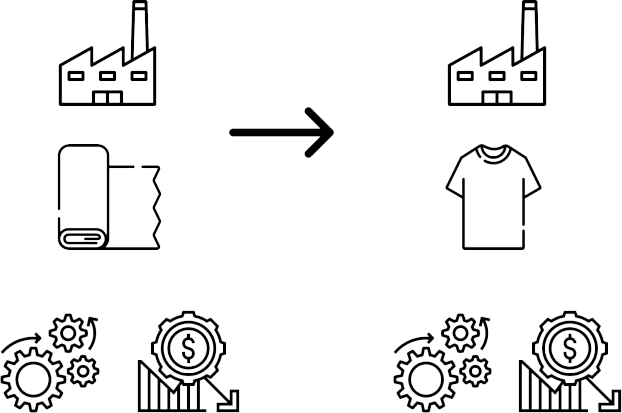
\includegraphics[width=0.45\textwidth,height=\textheight]{_000_images/001_image3.png}
\end{center}
\end{frame}

\begin{frame}{}
\phantomsection\label{section-5}
\begin{itemize}
\item
  How is measure?

  \begin{itemize}
  \item
    3 equivalent\footnote<.->{In practice, discrepancies may occur}
    approaches are used
    (\citeproc{ref-lequiller_understanding_2014}{Lequiller and Blades
    2014, 31})

    \begin{itemize}
    \item
      \textbf{Output/Production approach}: adding the aggregate value of
      all the production units in a territory, plus taxes minus
      subsidies on products
    \item
      \textbf{Income approach}: adding all the incomes that are
      perceived because of the contribution to the production process
    \item
      \textbf{Expenditure/Final demand approach}: adding all uses that
      firms, non-profit institutions, government bodies, households and
      the external sector give to production
    \end{itemize}
  \item
    Gross Domestic Product is a flow so is measured over a period of
    time. Usually you can find information about this varible in an
    monthly, quarterly or yearly periodicity
  \item
    Initially Gross Domestic Product is expressed in \textbf{current}
    Local Currency Units (LCU)
  \end{itemize}
\end{itemize}
\end{frame}

\begin{frame}{}
\phantomsection\label{section-6}
\begin{table}

\caption{\label{tbl-output-approach}Output/Production approach
(Colombia, 2024-Q1)}

\centering{

\centering\begingroup\fontsize{4.8}{6.8}\selectfont

\begin{threeparttable}
\begin{tabular}{>{\raggedright\arraybackslash}p{3.4in}>{\raggedleft\arraybackslash}p{0.8in}}
\toprule
\textbf{Concepto} & \textbf{Miles de Millones - COP\textsuperscript{a}}\\
\midrule
Agricultura, ganadería, caza, silvicultura y pesca & 34380\\
Explotación de minas y canteras & 16982\\
Industrias manufactureras & 40069\\
Suministro de electricidad, gas, vapor y aire acondicionado; Distribución de agua; evacuación y tratamiento de aguas residuales, gestión de desechos y actividades de saneamiento ambiental & 18092\\
Construcción & 16319\\
\addlinespace
Comercio al por mayor y al por menor; reparación de vehículos automotores y motocicletas; Transporte y almacenamiento; Alojamiento y servicios de comida & 76717\\
Información y comunicaciones & 9230\\
Actividades financieras y de seguros & 16857\\
Actividades inmobiliarias & 30166\\
Actividades profesionales, científicas y técnicas; Actividades de servicios administrativos y de apoyo & 25731\\
\addlinespace
Administración pública y defensa; planes de seguridad social de afiliación obligatoria; Educación; Actividades de atención de la salud humana y de servicios sociales & 56790\\
Actividades artísticas, de entretenimiento y recreación y otras actividades de servicios; Actividades de los hogares individuales en calidad de empleadores; actividades no diferenciadas de los hogares individuales como productores de bienes y servicios para uso propio & 14784\\
\cellcolor[HTML]{18BC9C}{Valor agregado bruto} & \cellcolor[HTML]{18BC9C}{356117}\\
\cellcolor[HTML]{CCBE93}{Impuestos menos subvenciones sobre los productos} & \cellcolor[HTML]{CCBE93}{42816}\\
\cellcolor[HTML]{e31a1c}{Producto interno bruto} & \cellcolor[HTML]{e31a1c}{398933}\\
\bottomrule
\end{tabular}
\begin{tablenotes}
\item Source: DANE - Cuentas Nacionales Trimestrales - Producto Interno Bruto desde el enfoque de la producción a precios corrientes - Cuadro 1 Datos originales
\item Last update: 2024-05-15
\item[a] Preliminary data at current prices
\end{tablenotes}
\end{threeparttable}
\endgroup{}

}

\end{table}%
\end{frame}

\begin{frame}{}
\phantomsection\label{section-7}
\begin{table}

\caption{\label{tbl-income-approach}Income approach (Colombia, 2024-Q1)}

\centering{

\centering\begingroup\fontsize{7}{9}\selectfont

\begin{threeparttable}
\begin{tabular}{>{\raggedright\arraybackslash}p{2in}>{\raggedleft\arraybackslash}p{2in}}
\toprule
\textbf{Concepto} & \textbf{Miles de Millones - COP\textsuperscript{a}}\\
\midrule
Remuneración de los asalariados & 127088\\
\cellcolor[HTML]{CCBE93}{Impuestos menos subvenciones} & \cellcolor[HTML]{CCBE93}{66294}\\
Excedente Bruto de Explotación & 122718\\
Ingreso Mixto & 82833\\
\cellcolor[HTML]{e31a1c}{Producto Interno Bruto} & \cellcolor[HTML]{e31a1c}{398933}\\
\bottomrule
\end{tabular}
\begin{tablenotes}
\item Source: DANE - Cuentas Nacionales Trimestrales - PIB por Ingreso - S1 Total Economía
\item Last update: 2024-06-28
\item[a] Preliminary data at current prices
\end{tablenotes}
\end{threeparttable}
\endgroup{}

}

\end{table}%
\end{frame}

\begin{frame}{}
\phantomsection\label{section-8}
\begin{table}

\caption{\label{tbl-expenditure-approach}Expenditure/Final demand
approach (Colombia, 2024-Q1)}

\centering{

\centering\begingroup\fontsize{7}{9}\selectfont

\begin{threeparttable}
\begin{tabular}{>{\raggedright\arraybackslash}p{2.6in}>{\raggedleft\arraybackslash}p{1.5in}}
\toprule
\textbf{Concepto} & \textbf{Miles de Millones - COP\textsuperscript{a}}\\
\midrule
Gasto de consumo final individual de los hogares y las ISFLH\textsuperscript{b} & 297141\\
Gasto de consumo final del gobierno general & 49385\\
Formación bruta de capital & 67943\\
Exportaciones & 60029\\
\cellcolor[HTML]{FF7F00}{Importaciones} & \cellcolor[HTML]{FF7F00}{75565}\\
\addlinespace
\cellcolor[HTML]{e31a1c}{Producto Interno Bruto} & \cellcolor[HTML]{e31a1c}{398933}\\
\bottomrule
\end{tabular}
\begin{tablenotes}
\item Source: DANE - Cuentas Nacionales Trimestrales - Producto Interno Bruto desde el enfoque del gasto a precios corrientes - Cuadro 1 Datos originales
\item Last update: 2024-05-15
\item[a] Preliminary data at current prices
\item[b] Instituciones sin fines de lucro que sirven a los hogares
\end{tablenotes}
\end{threeparttable}
\endgroup{}

}

\end{table}%
\end{frame}

\begin{frame}{}
\phantomsection\label{section-9}
\begin{itemize}
\item
  What adjustments are applied?\footnote<.->{For an introduction of the
    first 3 adjustments check out
    (\citeproc{ref-hyndman_forecasting_2021}{Hyndman and Athanasopoulos
    2021, chap. 3}, Section 3.1 Transformations and adjustments)}

  \begin{itemize}
  \item
    \textbf{Inflation adjustments}

    \begin{itemize}
    \tightlist
    \item
      GDP is expressed in \textbf{constant} Local Currency Units (LCU)
    \end{itemize}
  \item
    \textbf{Season and calendar adjustments}

    \begin{itemize}
    \tightlist
    \item
      In Colombia this is applied to quarterly GDP
      (\citeproc{ref-dane_cuentas_2018}{DANE 2018})
    \end{itemize}
  \item
    \textbf{Population adjustments}

    \begin{itemize}
    \tightlist
    \item
      GDP is expressed in per capita terms
    \end{itemize}
  \item
    \textbf{Purchase Power Parity (PPP) adjustment}

    \begin{itemize}
    \tightlist
    \item
      It is used only to make international comparisons and it is led by
      the International Comparison Program (ICP)
    \end{itemize}
  \end{itemize}
\end{itemize}
\end{frame}

\begin{frame}{}
\phantomsection\label{section-10}
\begin{itemize}
\tightlist
\item
  An inflation adjustment is necessary because an arbitrary quantity of
  local currency units don't have the same purchase power in different
  periods
\end{itemize}

\begin{center}
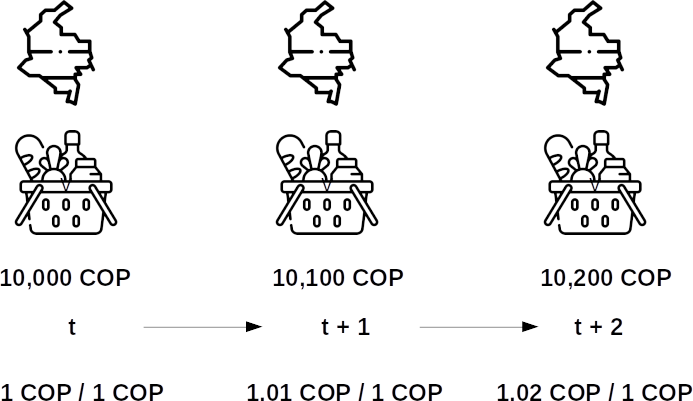
\includegraphics[width=0.6\textwidth,height=\textheight]{_000_images/002_image1.png}
\end{center}
\end{frame}

\begin{frame}{}
\phantomsection\label{section-11}
\begin{figure}

\centering{

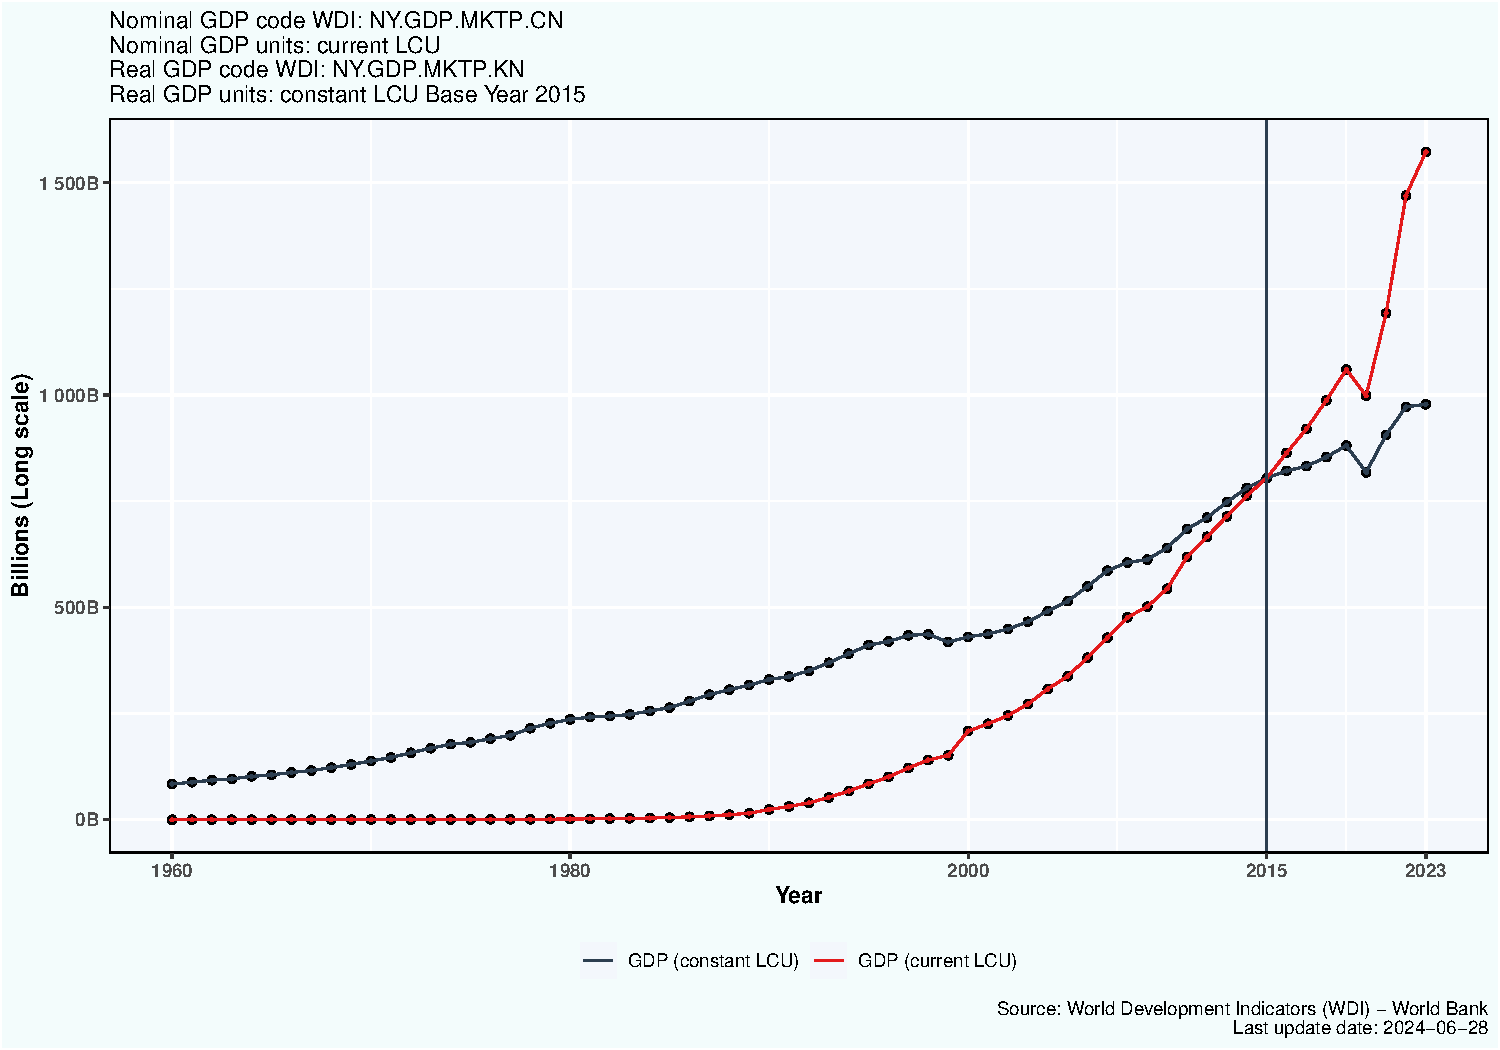
\includegraphics[width=0.85\textwidth,height=\textheight]{002_production_income_I_files/figure-beamer/fig-nominal-real-gdp-col-1.pdf}

}

\caption{\label{fig-nominal-real-gdp-col}Nominal and real GDP Colombia}

\end{figure}%
\end{frame}

\begin{frame}{}
\phantomsection\label{section-12}
\begin{itemize}
\tightlist
\item
  Some countries have more population than others so they can produce
  more. Therefore it is necessary to express the GDP per inhabitant
\end{itemize}

\begin{center}

\includegraphics[width=0.5\textwidth,height=\textheight]{_000_images/002_image2.png}
\end{center}
\end{frame}

\begin{frame}{}
\phantomsection\label{section-13}
\begin{figure}

\centering{

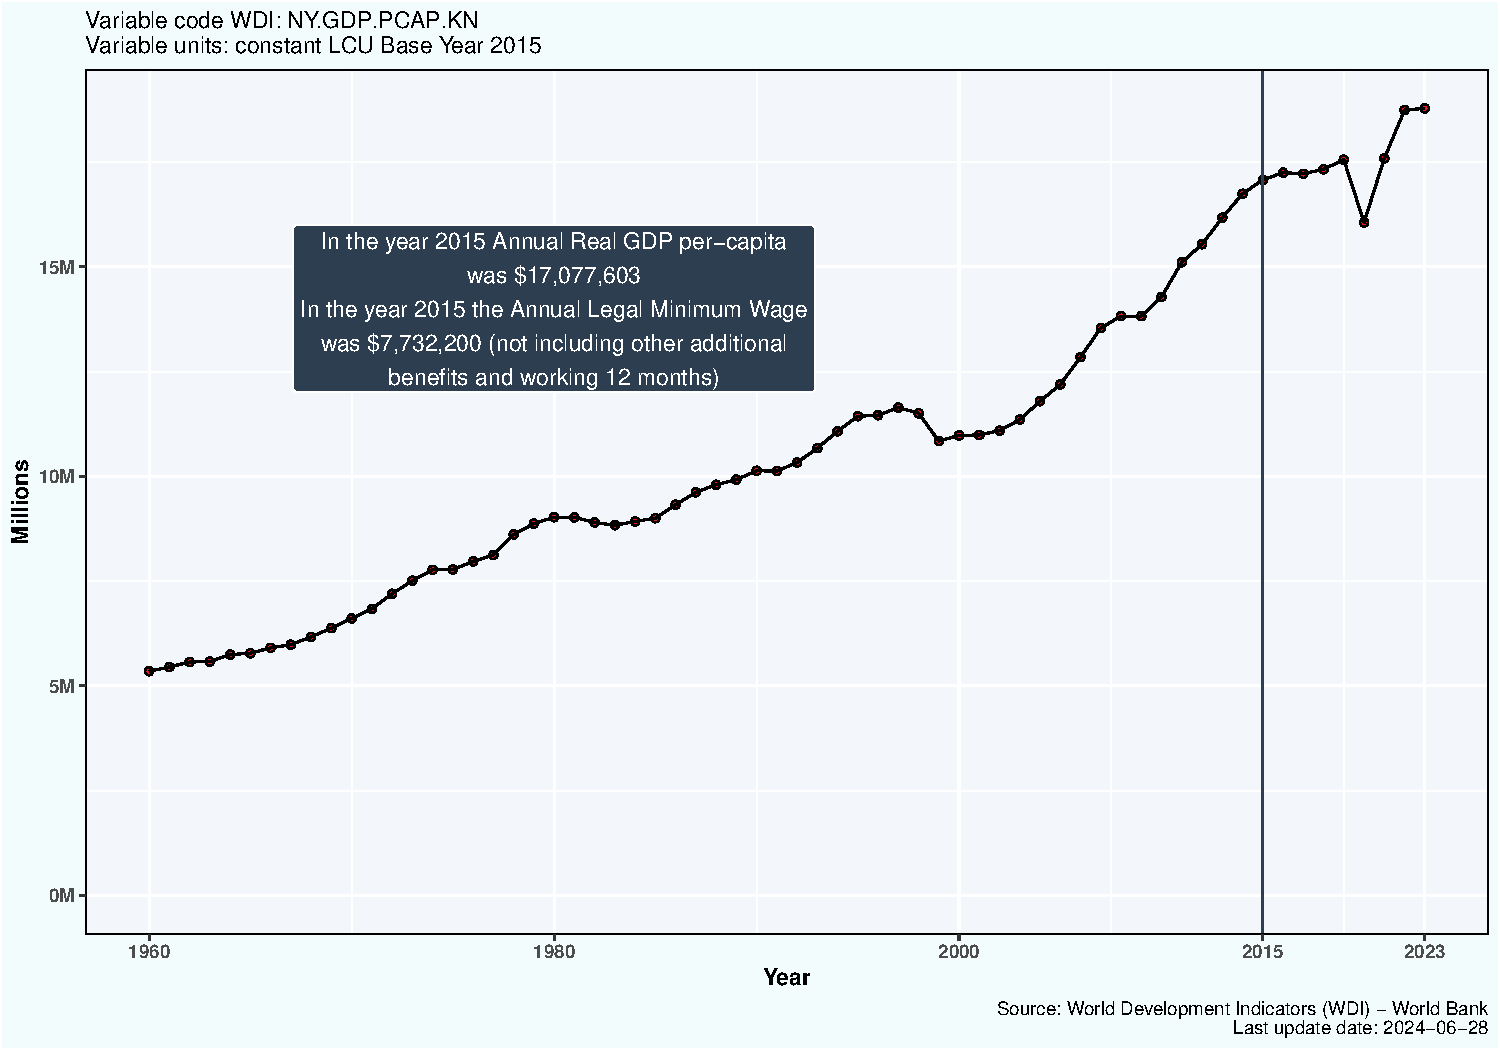
\includegraphics[width=0.85\textwidth,height=\textheight]{002_production_income_I_files/figure-beamer/fig-real-gdp-pc-col-1.pdf}

}

\caption{\label{fig-real-gdp-pc-col}Real GDP per-capita Colombia}

\end{figure}%
\end{frame}

\begin{frame}{}
\phantomsection\label{section-14}
\begin{itemize}
\item
  Purchasing power parity

  \begin{itemize}
  \tightlist
  \item
    The amount of products that 1 local currency unit of an economy can
    buy in another economy
  \end{itemize}
\end{itemize}

\begin{center}
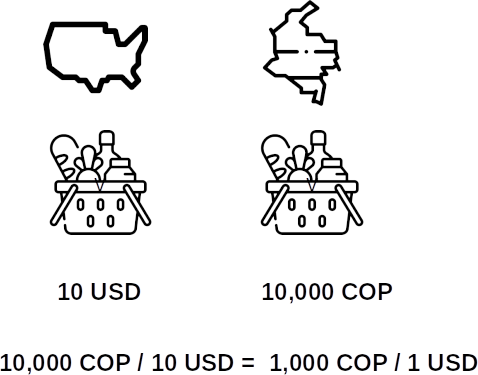
\includegraphics[width=0.5\textwidth,height=\textheight]{_000_images/002_image3.png}
\end{center}
\end{frame}

\begin{frame}{}
\phantomsection\label{section-15}
\begin{figure}

\centering{

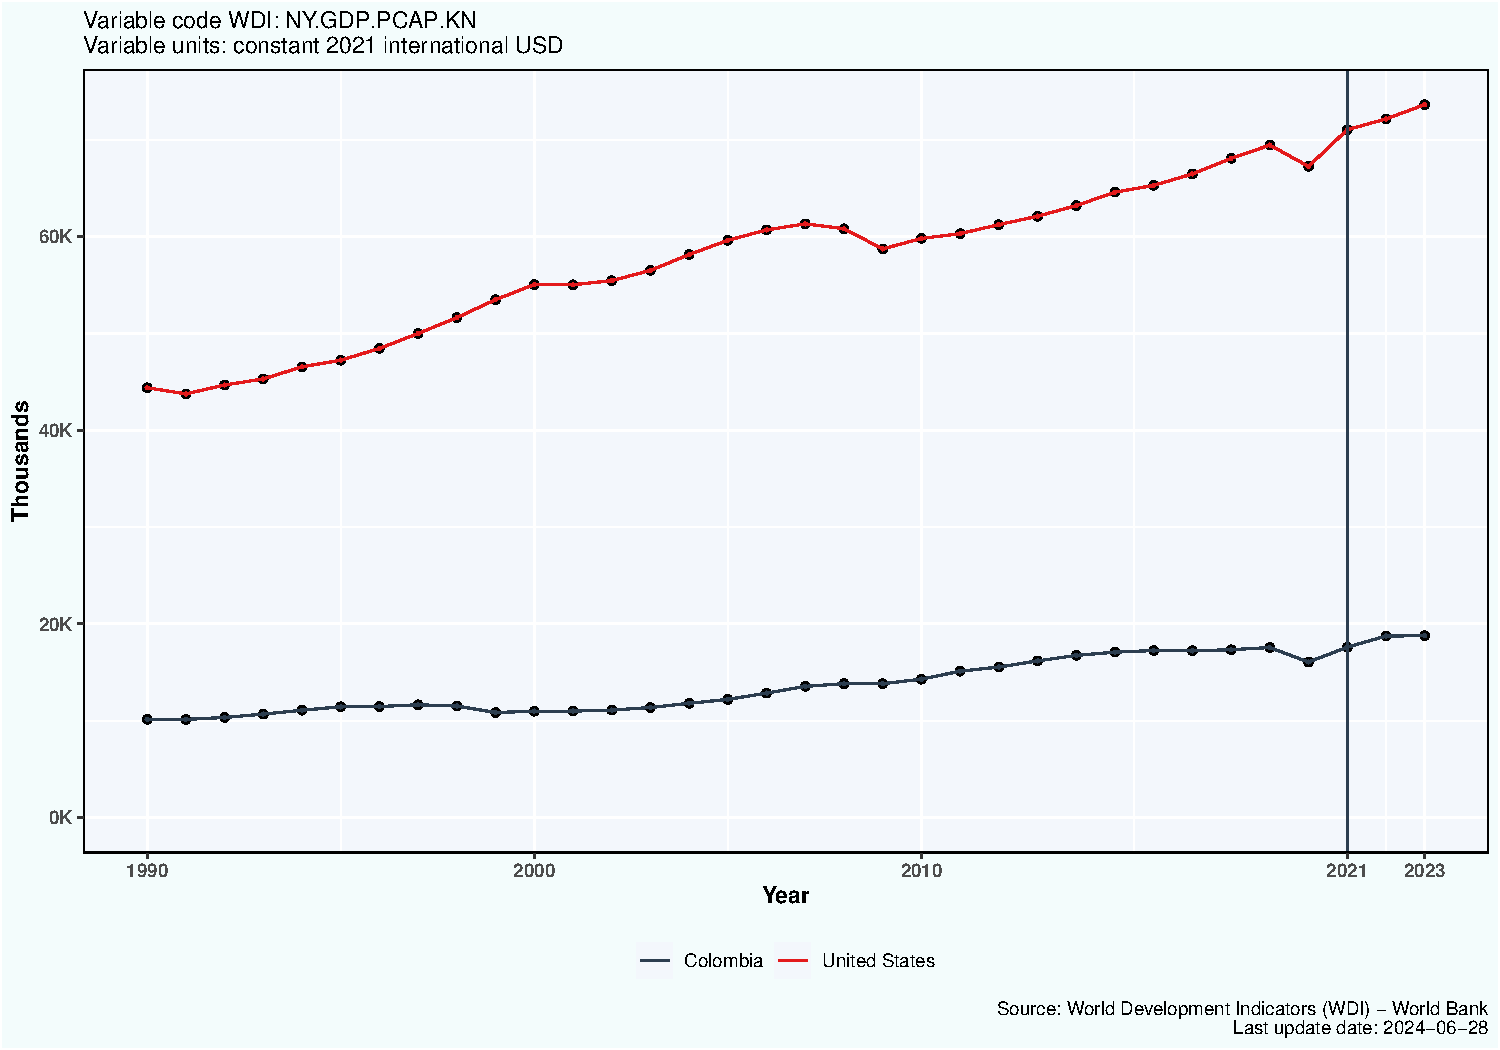
\includegraphics[width=0.85\textwidth,height=\textheight]{002_production_income_I_files/figure-beamer/fig-real-gdp-pc-ppp-col-usa-1.pdf}

}

\caption{\label{fig-real-gdp-pc-ppp-col-usa}GDP per-capita purchasing
power parity for Colombia and USA}

\end{figure}%
\end{frame}

\section{Economic Growth}\label{economic-growth}

\begin{frame}{}
\phantomsection\label{section-16}
\begin{itemize}
\item
  The most common metric used to measure economic growth is the annual
  percent growth of real GDP per capita.

  \begin{itemize}
  \tightlist
  \item
    If the periodicity of real GDP per capita is \textbf{yearly} and we
    don't want to make international comparisons the formula is:
  \end{itemize}
\end{itemize}

\[\frac{\text{GDP per capita constant LCU}_t - \text{GDP per capita constant LCU}_{t-1}}{\text{GDP per capita constant LCU}_{t-1}} \times 100\]
\end{frame}

\begin{frame}{}
\phantomsection\label{section-17}
\begin{itemize}
\item
  The most common metric used to measure economic growth is the annual
  percent growth of real GDP per capita.

  \begin{itemize}
  \tightlist
  \item
    If the periodicity of real GDP per capita is \textbf{quarterly} and
    we don't want to make international comparisons the formula is:
  \end{itemize}
\end{itemize}

\[\frac{\text{GDP per capita constant LCU}_t - \text{GDP per capita constant LCU}_{t-4}}{\text{GDP per capita constant LCU}_{t-4}} \times 100\]
\end{frame}

\begin{frame}{}
\phantomsection\label{section-18}
\begin{figure}

\centering{

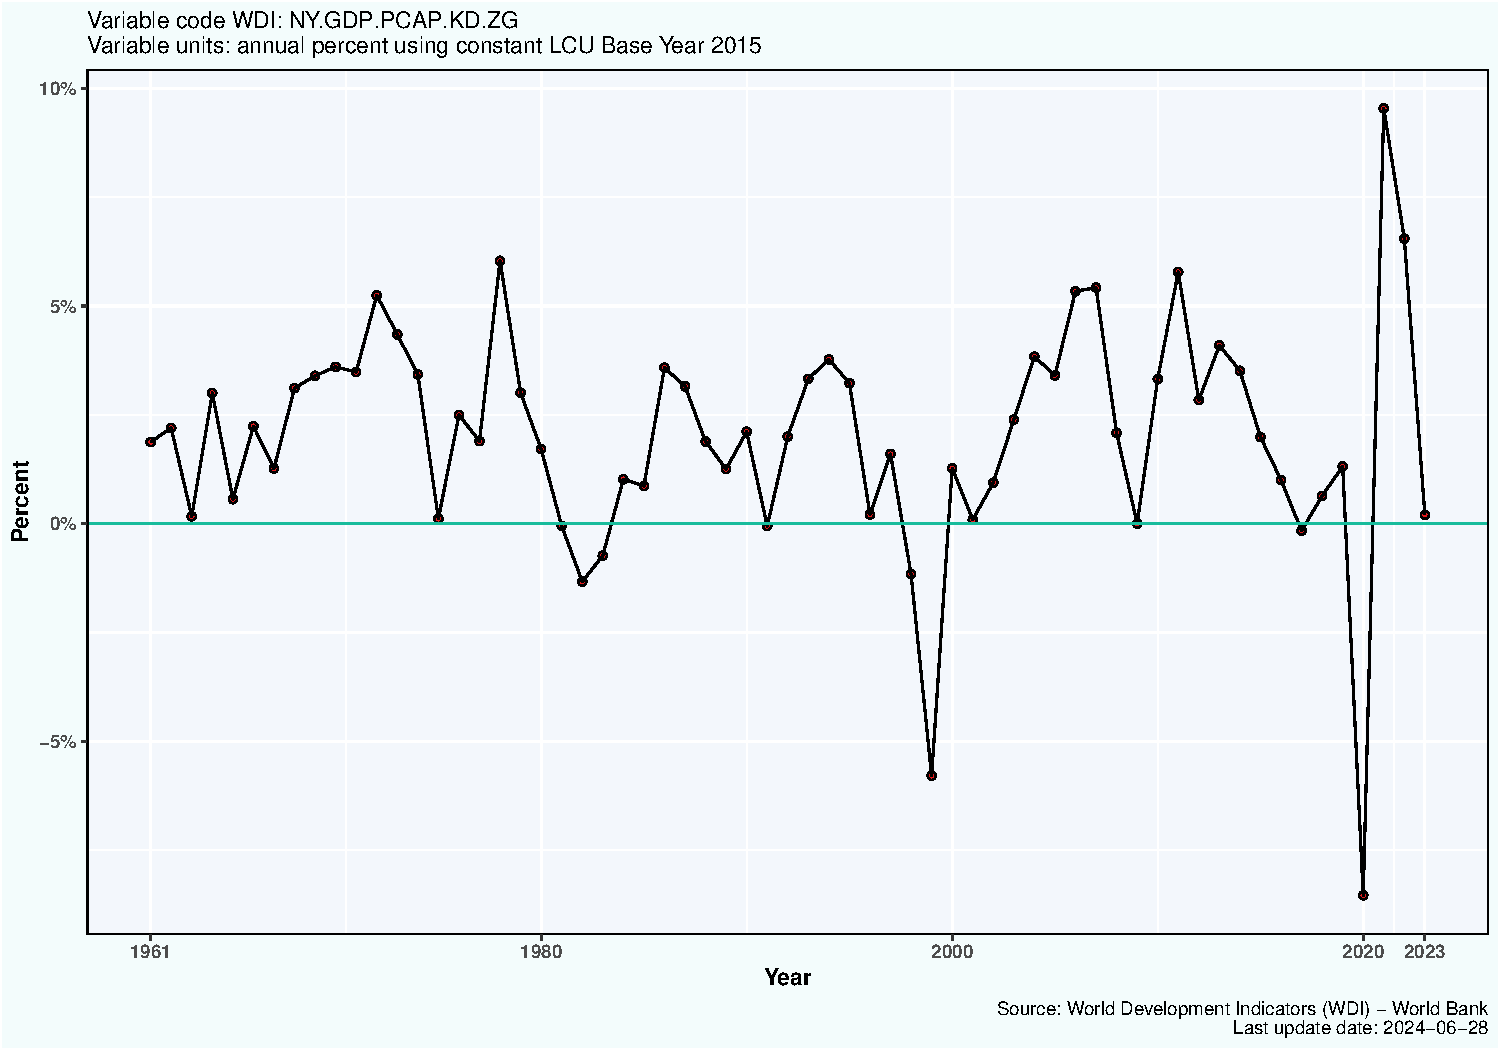
\includegraphics[width=0.85\textwidth,height=\textheight]{002_production_income_I_files/figure-beamer/fig-growth-real-gdp-pc-col-usa-1.pdf}

}

\caption{\label{fig-growth-real-gdp-pc-col-usa}Growth real GDP
per-capita Colombia}

\end{figure}%
\end{frame}

\section{Acknowledgments}\label{acknowledgments}

\begin{frame}{}
\phantomsection\label{section-19}
\begin{itemize}
\item
  To my family that supports me
\item
  To the taxpayers of Colombia and the
  \href{https://www.umng.edu.co/estudiante}{\textbf{UMNG students}} who
  pay my salary
\item
  To the \href{https://www.business-science.io/}{\textbf{Business
  Science}} and \href{https://www.rfordatasci.com/}{\textbf{R4DS Online
  Learning}} communities where I learn
  \href{https://www.r-project.org/about.html}{\textbf{R}} and
  \href{https://www.python.org/about/}{\textbf{\(\pi\)-thon}}
\item
  To the \href{https://www.r-project.org/contributors.html}{\textbf{R
  Core Team}}, the creators of
  \href{https://rstudio.com/products/rstudio/}{\textbf{RStudio IDE}},
  \href{https://quarto.org/}{\textbf{Quarto}} and the authors and
  maintainers of the packages
  \href{https://CRAN.R-project.org/package=tidyverse}{\textbf{tidyverse}},
  \href{https://CRAN.R-project.org/package=readxl}{\textbf{readxl}},
  \href{https://CRAN.R-project.org/package=knitr}{\textbf{knitr}},
  \href{https://CRAN.R-project.org/package=kableExtra}{\textbf{kableExtra}},
  \href{https://CRAN.R-project.org/package=tidyquant}{\textbf{tidyquant}},
  \href{https://CRAN.R-project.org/package=wbstats}{\textbf{wbstats}}
  and
  \href{https://CRAN.R-project.org/package=tinytex}{\textbf{tinytex}}
  for allowing me to access these tools without paying for a license
\item
  To the \href{https://www.kernel.org/category/about.html}{\textbf{Linux
  kernel community}} for allowing me the possibility to use some
  \href{https://static.lwn.net/Distributions/}{\textbf{Linux
  distributions}} as my main
  \href{https://en.wikipedia.org/wiki/Operating_system}{\textbf{OS}}
  without paying for a license
\end{itemize}
\end{frame}

\begin{frame}{}
\phantomsection\label{section-20}
\begin{itemize}
\tightlist
\item
  To the icon designers
  \href{https://www.flaticon.com/authors/becris}{\textbf{Brecris}},
  \href{https://www.flaticon.com/authors/freepik}{\textbf{Freepik}},
  \href{https://www.flaticon.com/authors/iconixar}{\textbf{Iconixar}},
  \href{https://www.flaticon.com/authors/monkik}{\textbf{Monkik}} and
  \href{https://www.flaticon.com/authors/eucalyp}{\textbf{Eucalyp}} from
  \href{https://www.flaticon.com/}{\textbf{Flaticon}} for letting me use
  their work in this presentation as a free user
\end{itemize}
\end{frame}

\section*{References}\label{references}
\addcontentsline{toc}{section}{References}

\begin{frame}[allowframebreaks]{References}
\phantomsection\label{refs}
\begin{CSLReferences}{1}{0}
\bibitem[\citeproctext]{ref-cardenas_introduccion_2020}
Cardenas, Mauricio. 2020. \emph{Introducción a La {Economía}
{Colombiana}}. 4th ed. Alfaomega.

\bibitem[\citeproctext]{ref-dane_cuentas_2018}
DANE. 2018. {``Cuentas {Nacionales} {Trimestrales} {Ajuste}
{Estacional}.''}
\url{https://www.dane.gov.co/files/investigaciones/boletines/pib/ajuste-estacional-pib.pdf}.

\bibitem[\citeproctext]{ref-hyndman_forecasting_2021}
Hyndman, Robin John, and George Athanasopoulos. 2021. \emph{Forecasting:
{Principles} and {Practice} (3rd Ed)}. \url{https://Otexts.com/fpp3/}.

\bibitem[\citeproctext]{ref-lequiller_understanding_2014}
Lequiller, François, and Derek Blades. 2014. \emph{Understanding
{National} {Accounts}: {Second} {Edition}}. OECD.
\url{https://doi.org/10.1787/9789264214637-en}.

\end{CSLReferences}
\end{frame}




\end{document}
